\documentclass[11pt]{article}
\usepackage[french]{babel}

\usepackage[utf8]{inputenc}
\usepackage{palatino}
\usepackage[T1]{fontenc}


\usepackage{url}
\usepackage{amsmath}

\usepackage[top=2cm,bottom=2cm,left=2.1cm,right=2.1cm,headsep=10pt,a4paper]{geometry}
\usepackage{fancyhdr}


\usepackage{graphicx,float} % figure et placement de figure
\usepackage{listings} %%inclusion de programmes

\lstset{
language=C++,
basicstyle=\ttfamily\small, %
identifierstyle=\color{black}, %
keywordstyle=\color{blue}, %
stringstyle=\color{blue}, %
commentstyle=\it\color{green}, %
}

\usepackage{xcolor}

\pagestyle{fancy}
\lhead{}
\chead{\fontsize{10}{10}{M2IM - UCBL - 2014/2015}}
\rhead{}

\lfoot{}
\cfoot{\thepage}
\rfoot{}


\renewcommand{\headrulewidth}{0pt}
\renewcommand{\footrulewidth}{0pt}
%11006689

 \author{\fontsize{14}{14}{Aurélien CHEMIER 10908892 et Romane LHOMME 11006689}}
 \title{\fontsize{16}{16}{{\bf Analyse, aquisition et traitement d’image \\ TP1}}}
 \date{\fontsize{11}{11}{\today}}

\begin{document}

\thispagestyle{empty}
\maketitle

\newpage

\section{Introduction}

	Dans le cadre de ce projet d’analyse d’image, nous devons implémenter une méthode de détection de contours, à l’aide des filtres vus en cours. 
	Ensuite, une étape de traitement et d'affinage des contours  sera effectuer afin d'avoir un meilleur résultat.
	Ce rapport à pour but de présenter et d'expliquer nos choix lors de ces différentes étapes.

	\section{Technologies utilisées}

	Ce programme de detection de contour a été fait en C++ qui est un langage objet que nous avons l'habitude d'utiliser.

	Pour manipuler les images, nous avons choisi d'utiliser OpenCV, une bibliothèque graphique spécialisée dans le traitement d'image en temps réel.
	Cette librairie a plusieurs avantages :
	\begin{itemize}
		\item Elle est gratuite.
		\item Elle permet une gestion simple des images (lecture, écriture, sauvegarde...).
	\end{itemize}

	L'utilisation de notre programme se fait en ligne de commande.

	Tous nos tests ont été fait sur l'image "Lena", un classique du traitement d'image.

	\begin{figure}[H]
		\centering
		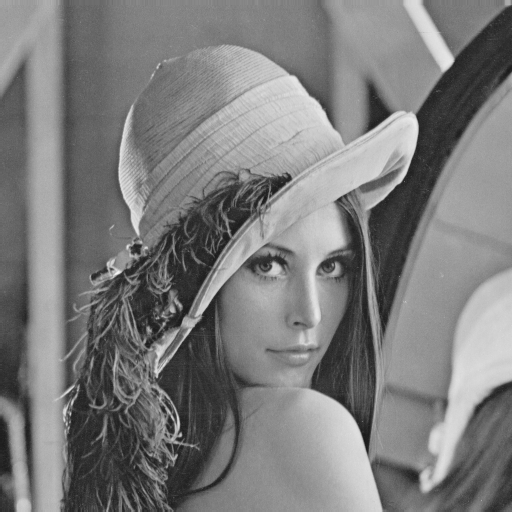
\includegraphics[scale=0.20]{Image/lena.png}
		\caption{Lena}
		\label{fig:Lena}
	\end{figure}

\section{Détection des contours}
	
	L'étape de détection des contours se fait uniquement sur des images en niveaux de gris.

	Dans un premier temps, on procède au calcul du vecteur gradient en chaque point de l'image.
	La méthode demandée consiste à appliquer des opérateurs (ou masques) de convolution (tableau MxM).

	Pour chaque Pixel de l'image, on fait la somme du produit des pixels voisins avec la case du filtre correspndante, comme le montre le code suivant.
	\begin{lstlisting}[caption={Utilisation d'un masque de convolution 3x3},language=C++,label=utilisationMasque]
	for (i = 0; i < 3; ++i)
	{
		for (j = 0; j < 3; ++j)
		{ 
			gradient += p[i][j] * Filtre[i][j];	
		}
	}
	\end{lstlisting}

	Le pixel sur lequel s'applique le filtre se situe au milieu de celui ci, ici en position 1,1.

	Le gradient est ensuite normalisé entre 0 et 255 et devient la valeur du pixel courant dans l'image filtrée.

	Tous les filtres appliqués dans ce TPs sont de dimension 3x3.
[H]
	Différents filtres peuvent être utilisés :  

	\begin{itemize}
		\item Prewitt

			\begin{tabular}{cccc}
				horizontal &
				$
				\begin{pmatrix}
					1 & 0 & -1 \\
					1 & 0 & -1 \\
					1 & 0 & -1
				\end{pmatrix}
				$
				&
				vertical &
				$
				\begin{pmatrix}
				1 & 1 & 1 \\
				0 & 0 & 0 \\
				-1 & -1 & -1
				\end{pmatrix}
				$
			\end{tabular}

		\item Sobel

			\begin{tabular}{cccc}
				horizontal &
				$
				\begin{pmatrix}
				1 & 0 & -1 \\
				2 & 0 & -2 \\
				1 & 0 & -1
				\end{pmatrix}
				$
				&
				vertical &
				$
				\begin{pmatrix}
				1 & 2 & 1 \\
				0 & 0 & 0 \\
				-1 & -2 & -1
				\end{pmatrix}
				$
			\end{tabular}

		\item Kisrch

			\begin{tabular}{cccc}
				horizontal &
				$
				\begin{pmatrix}
				-3 & -3 & 5 \\
				-3 & 0 & 5 \\
				-3 & -3 & 5
				\end{pmatrix}
				$
				&
				vertical &
				$
				\begin{pmatrix}
				-3 & -3 & -3 \\
				-3 & 0 & -3 \\
				5 & 5 & 5
				\end{pmatrix}
				$
			\end{tabular}
			
			\item D'autres masques peuvent être utilisés.
	\end{itemize}

	Ces différents filtres appliqués à Lena donnent : 

	\begin{figure}[H]
		\begin{minipage}[c]{.46\linewidth}
			\centering
			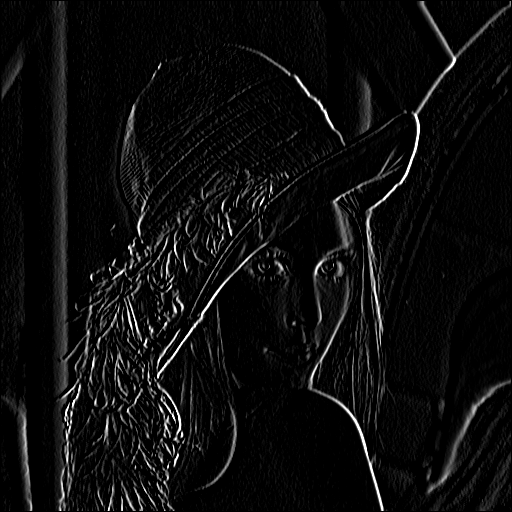
\includegraphics[scale=0.25]{Image/filtrePrewittHorizontal.png}
			\caption{Prewitt Horizontal}
			\label{fig:PrewittHorizontal}
		\end{minipage} \hfill
		\begin{minipage}[c]{.46\linewidth}
		\centering
			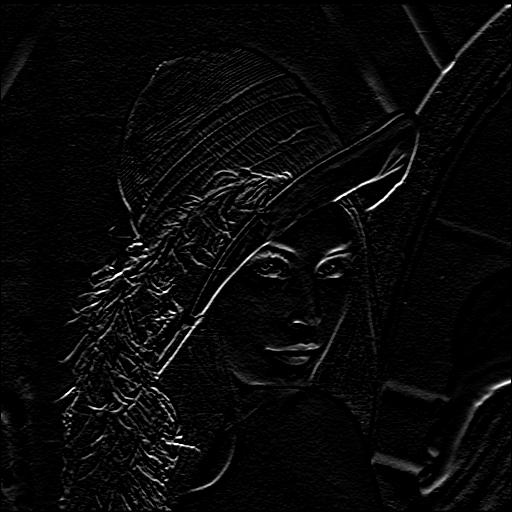
\includegraphics[scale=0.25]{Image/filtrePrewittVertical.png}
			\caption{Prewitt Vertical}
			\label{fig:PrewittVertical}
		\end{minipage}
	\end{figure}

	\begin{figure}[H]
		\begin{minipage}[c]{.46\linewidth}
			\centering
			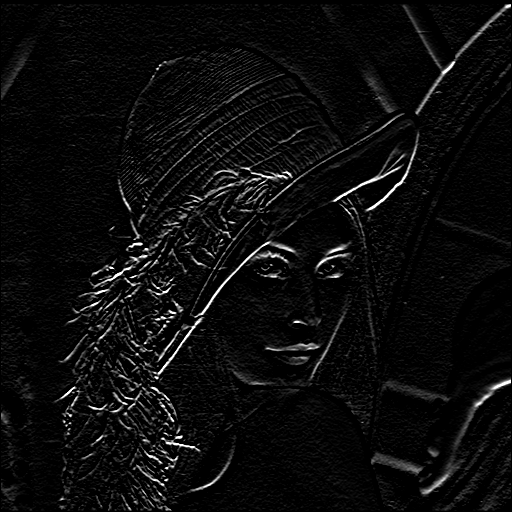
\includegraphics[scale=0.25]{Image/filtreSobelHorizontal.png}
			\caption{Sobel Horizontal}
			\label{fig:SobelHorizontal}
		\end{minipage} \hfill
		\begin{minipage}[c]{.46\linewidth}
		\centering
			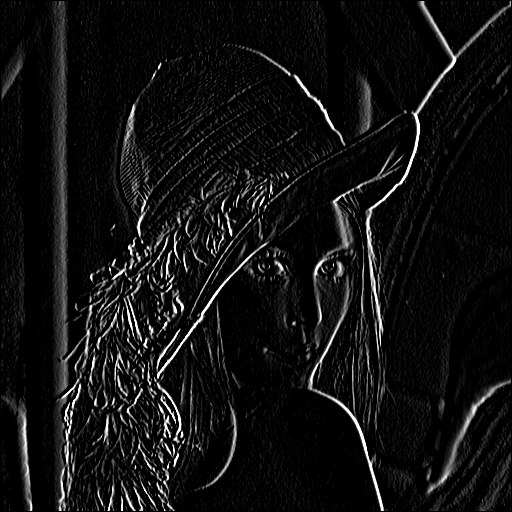
\includegraphics[scale=0.25]{Image/filtreSobelVertical.png}
			\caption{Sobel Vertical}
			\label{fig:SobelVertical}
		\end{minipage}
	\end{figure}

	\begin{figure}[H]
		\begin{minipage}[c]{.46\linewidth}
			\centering
			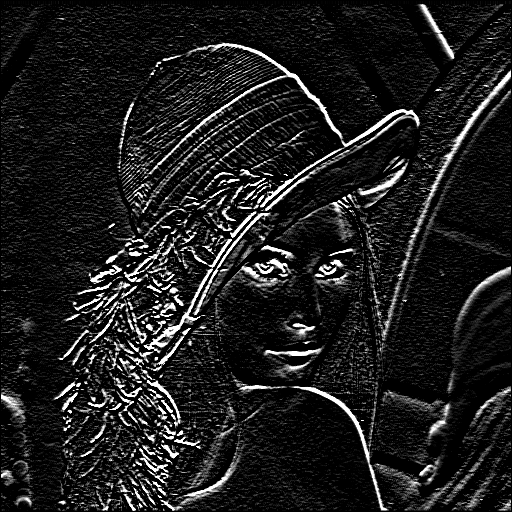
\includegraphics[scale=0.25]{Image/filtreKirshHorizontal.png}
			\caption{Kirsh Horizontal}
			\label{fig:KirshHorizontal}
		\end{minipage} \hfill
		\begin{minipage}[c]{.46\linewidth}
		\centering
			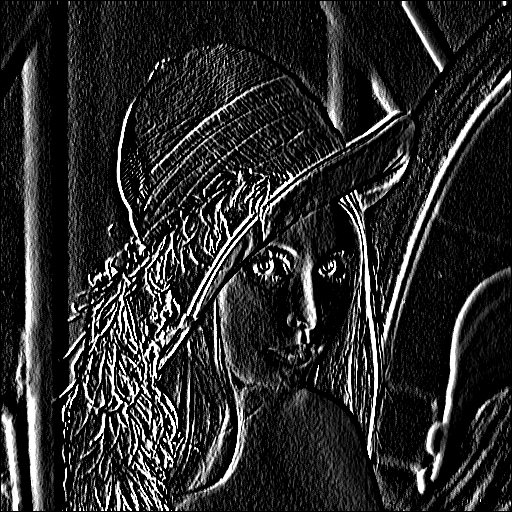
\includegraphics[scale=0.25]{Image/filtreKirshVertical.png}
			\caption{Kirsh Vertical}
			\label{fig:KirshVertical}
		\end{minipage}
	\end{figure}

	La complexité de cette méthode est de l’ordre \[w \times h\] avec:
	\begin{itemize}
		\item \textit{w} la largeur de l’image,
		\item \textit{h} la hauteur de l’image. 
	\end{itemize}

	\subsection{Filtrage bidirectionnel}

	Le filtrage bidirectionnel consiste à appliquer deux masque de convolutions sur la même image.
	La valeur du gradient devient: 
	\[G = \sqrt{GV^2 + GH^2}\]
	Avec 
	\begin{itemize}
		\item \textit{G} le gradient du filtre bidirectionnel,
		\item \textit{GV} le gradient du filtre vertical,
		\item \textit{GH} le gradient du filtre horizontal.
	\end{itemize}

	\begin{figure}[H]
		\begin{minipage}[c]{.46\linewidth}
			\centering
			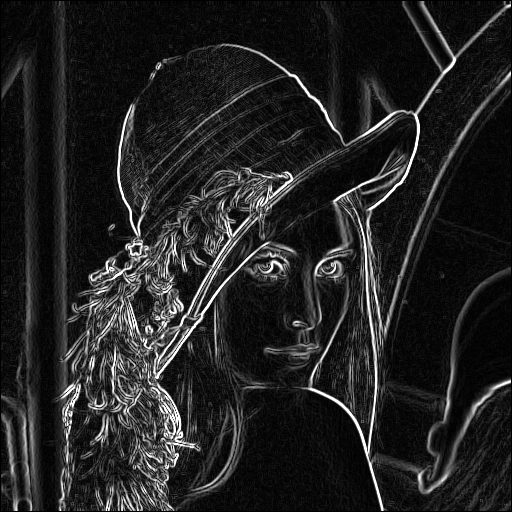
\includegraphics[scale=0.25]{Image/filtrePrewittBidirectionnel.png}
			\caption{Prewitt Bidirectionnel}
			\label{fig:PrewittBidirectionnel}
		\end{minipage} \hfill
		\begin{minipage}[c]{.46\linewidth}
		\centering
			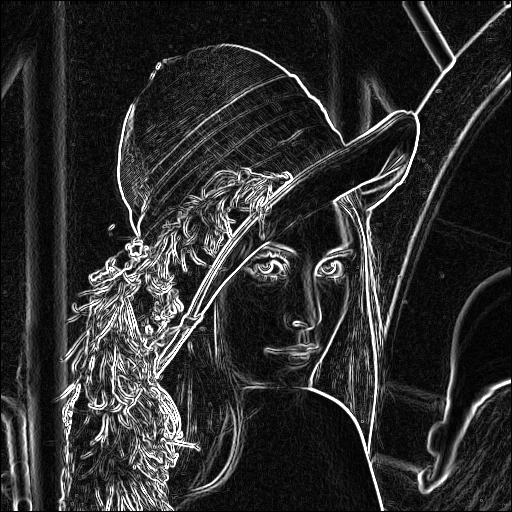
\includegraphics[scale=0.25]{Image/filtreSobelBidirectionnel.png}
			\caption{Sobel Bidirectionnel}
			\label{fig:SobelBidirectionnel}
		\end{minipage}
	\end{figure}

	\begin{figure}[H]
		\centering
		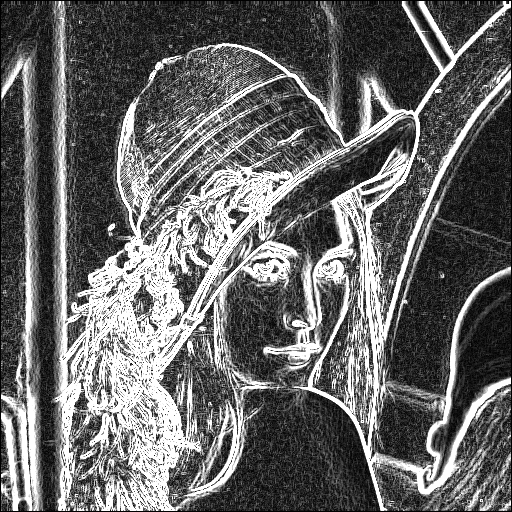
\includegraphics[scale=0.25]{Image/filtreKirshBidirectionnel.png}
		\caption{Kirsh Bidirectionnel}
		\label{fig:KirshBidirectionnel}
	\end{figure}

	L’avantage de cette méthode est que seul 2 filtres sont nécessaires pour calculer le gradient en 1 point. 
	Cependant elle peut être plus sensible au bruit que la méthode multidirectionelle.

	Comme les deux filtres sont calculé sur le même de l'image, la complexité est également de \[w \times h\].

	\subsection{Filtrage multidirectionnel}

	Pour le calcul du filtre multidirectionnel deux masques diagonaux sont rajoutés, voici ceux du filtre de Prewitt:
	\\
	\begin{tabular}{cccc}
		Diagonal gauche &
		$
		\begin{pmatrix}
			1 & 1 & 0 \\
			1 & 0 & -1 \\
			0 & -1 & -1
		\end{pmatrix}
		$
		& Diagonal droite &
		$
		\begin{pmatrix}
		0 & 1 & 1 \\
		-1 & 0 & 1 \\
		-1 & -1 & 0
		\end{pmatrix}
		$
	\end{tabular}

	Ces filtres donnent : 

	\begin{figure}[H]
		\begin{minipage}[c]{.46\linewidth}
			\centering
			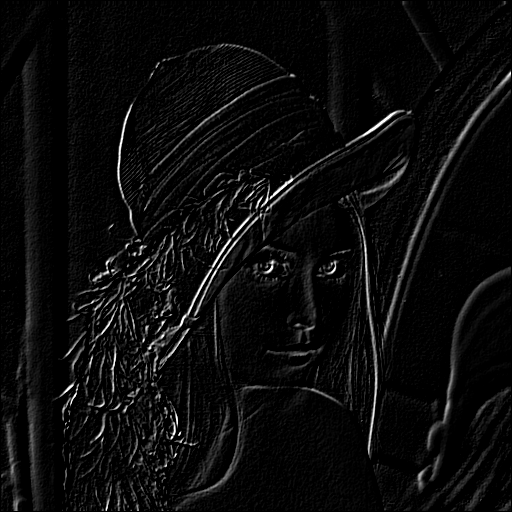
\includegraphics[scale=0.25]{Image/filtrePrewittDiagonalG.png}
			\caption{Prewitt Diagonal Gauche}
			\label{fig:PrewittDiagonalG}
		\end{minipage} \hfill
		\begin{minipage}[c]{.46\linewidth}
		\centering
			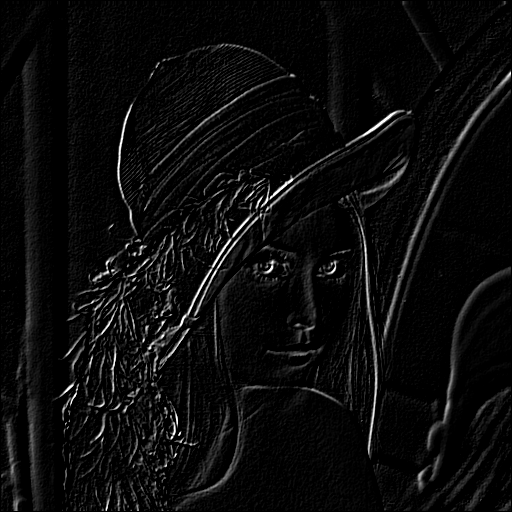
\includegraphics[scale=0.25]{Image/filtrePrewittDiagonalD.png}
			\caption{Prewitt Diagonal Droite}
			\label{fig:SobelDiagonalD}
		\end{minipage}
	\end{figure}

	Le filtre multidirectionnel calcule donc un filtre bidirectionnel avec les filtres diagonaux correspondants.

	\begin{figure}[H]
		\begin{minipage}[c]{.46\linewidth}
			\centering
			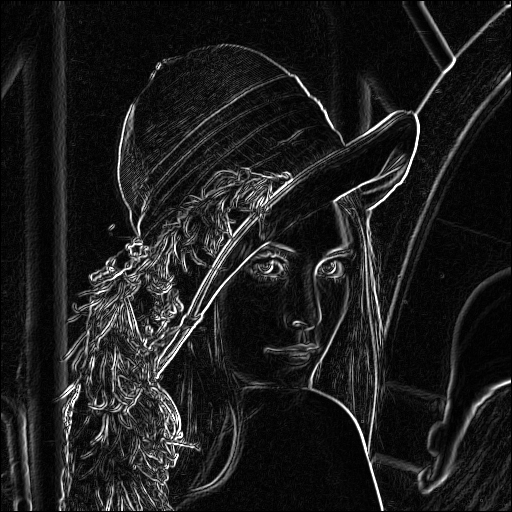
\includegraphics[scale=0.25]{Image/filtrePrewittMultidirectionnel.png}
			\caption{Prewitt Multidirectionnel}
			\label{fig:PrewittMultidirectionnel}
		\end{minipage} \hfill
		\begin{minipage}[c]{.46\linewidth}
		\centering
			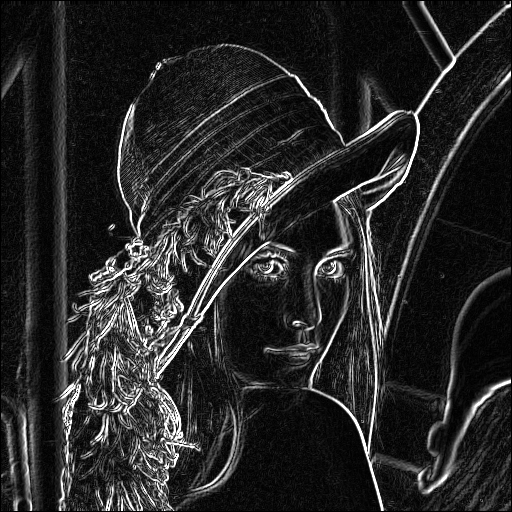
\includegraphics[scale=0.25]{Image/filtreSobelMultidirectionnel.png}
			\caption{Sobel Multidirectionnel}
			\label{fig:SobelMultidirectionnel}
		\end{minipage}
	\end{figure}

	\begin{figure}[H]
		\centering
		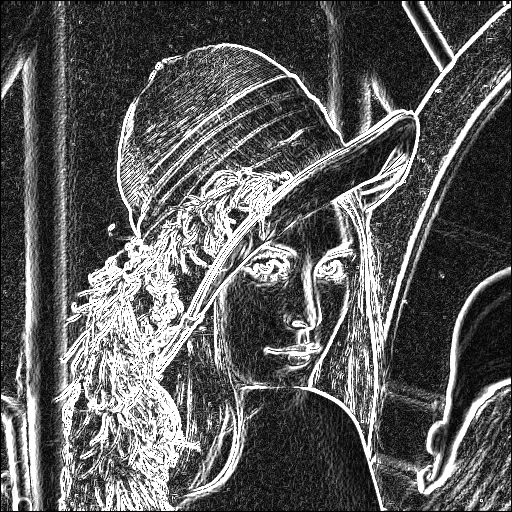
\includegraphics[scale=0.25]{Image/filtreKirshMultidirectionnel.png}
		\caption{Kirsh Multidirectionnel}
		\label{fig:KirshMultidirectionnel}
	\end{figure}

	Le calcul des masques se faisant toujours en un seul passage sur l'image, la complexité ne change pas.

	L'utilisation de plus de filtre permet de réduire le bruit sur la detection des contours. 
	Néanmoins, ce bruit est toujours présent, c'est pourquoi il faut passer à l'étape du seuillage.
 
\section{Seuillage}
	
	Le seuillage consiste à "filtrer" les pixels de l'image filtrer en fonction d'un seuil. 
	Si la valeur du pixel courant est inférieur au seuil, elle est passée à 0, sinon elle prend la valeur maximale (ici 255).

	Celui ci peut être déterminer de plusieurs manière.

	\subsection{Seuillage fixe}\label{fixe}

	Le seuil S est fixé et est commun à toute l'image. néanmoins il faut choisir une bonne valeur pour avoir un résultat correct.

	Les exemples ci-dessous ont été calculé sur un filtre de Prewitt multidirectionnel.
	\begin{figure}[H]
		\begin{minipage}[c]{.30\linewidth}
			\centering
			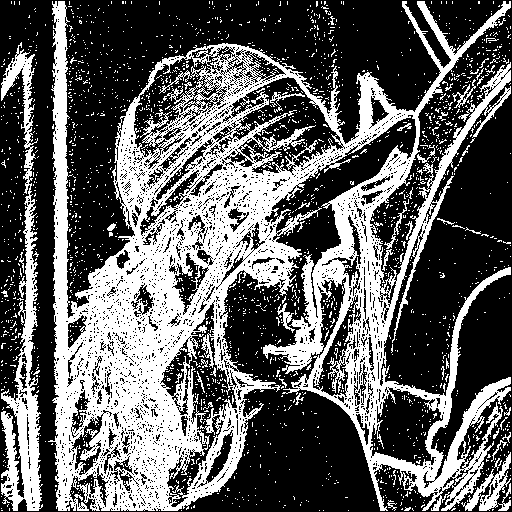
\includegraphics[scale=0.15]{Image/seuilFixe20.png}
			\caption{S = 20}
			\label{fig:seuilFixe20}
		\end{minipage} \hfill
		\begin{minipage}[c]{.30\linewidth}
			\centering
			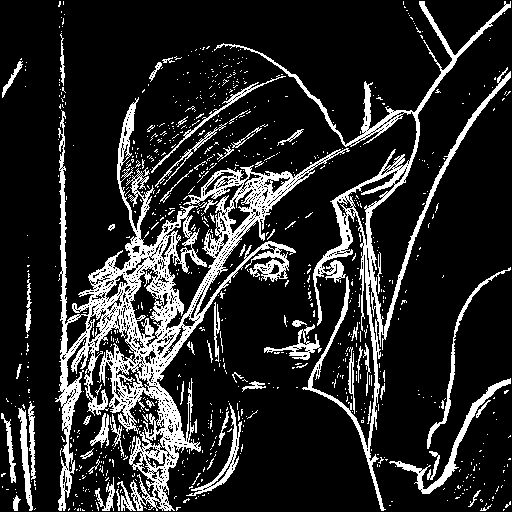
\includegraphics[scale=0.15]{Image/seuilFixe50.png}
			\caption{S = 50}
			\label{fig:seuilFixe50}
		\end{minipage} \hfill
		\begin{minipage}[c]{.30\linewidth}
			\centering
			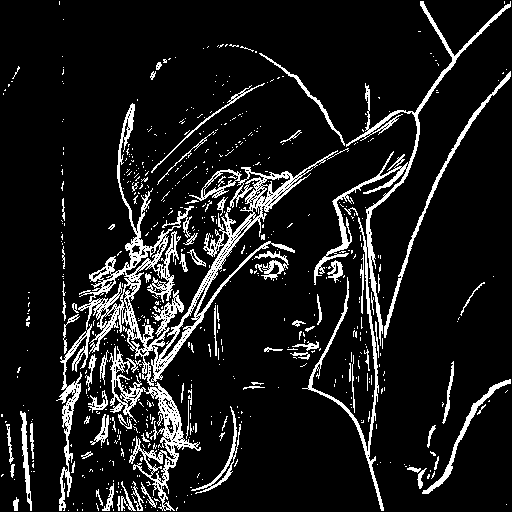
\includegraphics[scale=0.15]{Image/seuilFixe70.png}
			\caption{S = 70}
			\label{fig:seuilFixe70}
		\end{minipage}

		\begin{minipage}[c]{.30\linewidth}
			\centering
			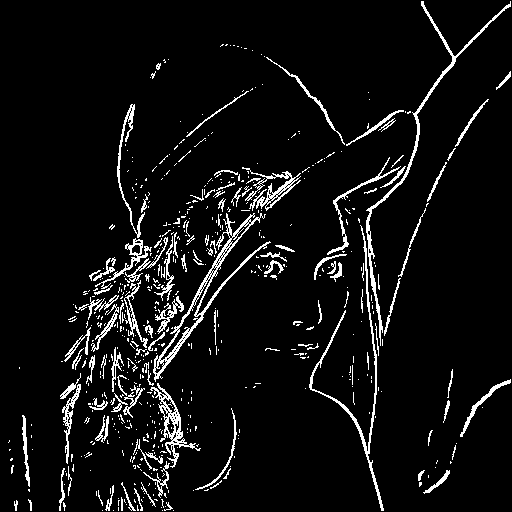
\includegraphics[scale=0.15]{Image/seuilFixe100.png}
			\caption{S = 100}
			\label{fig:SeuilFixe100}
		\end{minipage} \hfill
		\begin{minipage}[c]{.30\linewidth}
			\centering
			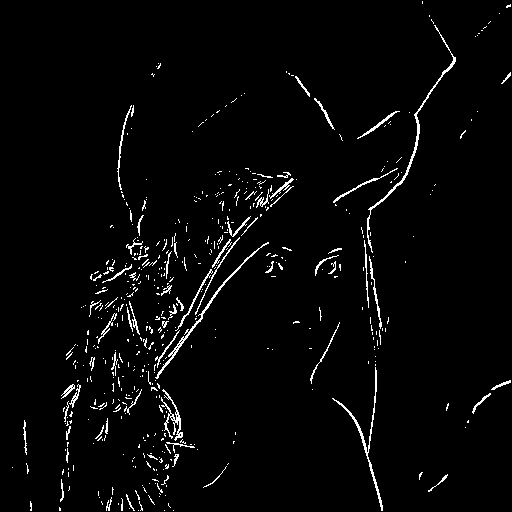
\includegraphics[scale=0.15]{Image/seuilFixe150.png}
			\caption{S = 150}
			\label{fig:seuilFixe150}
		\end{minipage} \hfill
		\begin{minipage}[c]{.30\linewidth}
			\centering
			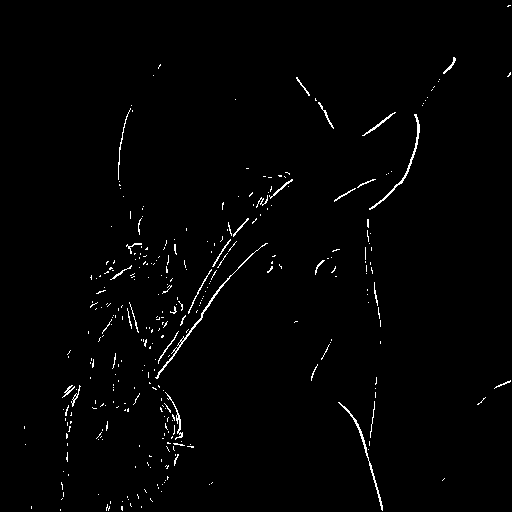
\includegraphics[scale=0.15]{Image/seuilFixe200.png}
			\caption{S = 200}
			\label{fig:seuilFixe200}
		\end{minipage}
	\end{figure}

	Pour des seuils très bas, on  remarque bien que le bruit est important (figure \ref{fig:seuilFixe20}).
	Au contraire, dans le cas de seuil élevé, certain contours sont effacés et l'image perd en précision (figure \ref{fig:seuilFixe150} et \ref{fig:seuilFixe200}).

	La compléxité de cette méthode est de \[w \times h\]

	\subsection{Seuillage global}

	Nous venons de voir que le choix du seuil est crucial dans le seuillage de l'image. 
	Il est rapidement contraignant de chercher "à la main" le seuil optimal pour une image.
	Le seuillage globale permet de determiner un seuil pour une image : il calcule la valeur moyenne des gradients de l'image et 
	prend cette moyenne comme seuil.

	\begin{figure}[H]
		\centering
		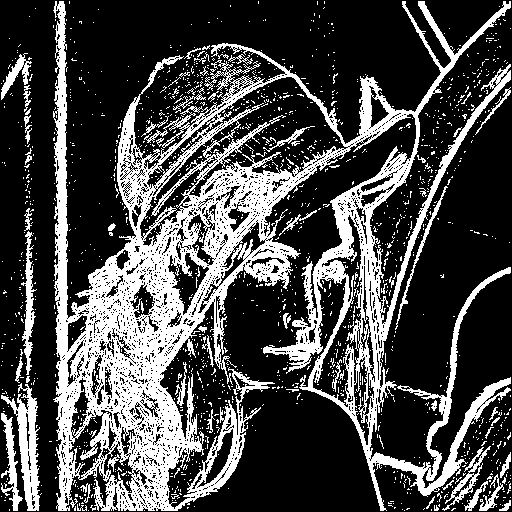
\includegraphics[scale=0.25]{Image/seuilGlobal.png}
		\caption{Seuillage Global de Prewitt multidirectionnel}
		\label{fig:seuilGlobal}
	\end{figure} 

	La complexité est plus grande car on effectue deux parcours de l’image: \[2 \times w \times x\]

	L’image contenant beaucoup de nuances de gris comme contours, le résultat contient beaucoup de "bruit" dans les contours.

	\subsection{Seuillage local}

	Le seuillage local calcule la moyenne des pixels voisins au pixel courant. 
	Une fois cette moyenne calculé, on la compare avec le pixel courant.

	\begin{figure}[H]
		\centering
		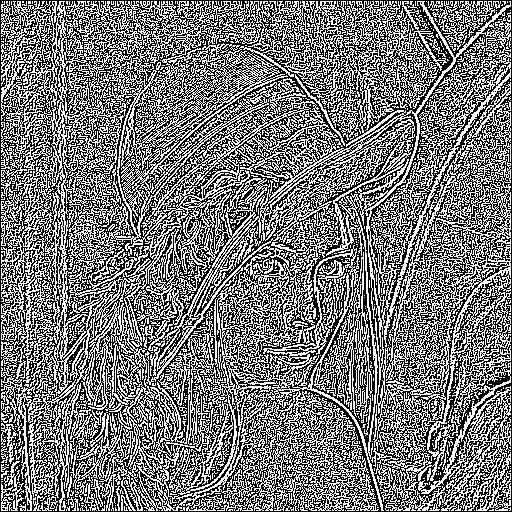
\includegraphics[scale=0.25]{Image/seuilLocal.png}
		\caption{Seuillage Local de Prewitt multidirectionnel}
		\label{fig:seuilLocal}
	\end{figure} 

	Le résultat est  bruité mais celui-ci a une précision supérieur à celle du seuil global. 
	En effet, on retrouve toute les courbes intacts dans l'image seuillée.

	La complexité est plus élevée a cause du calcul systématique de la moyenne locale: \[l^2 \times w \times x\]
	avec \textit{l} la taille de la zone où est calculé la moyenne.

	\subsection{Seuillage par Hysteresis}

	Dans le cas d'un seuillage par hysteresis, on utilise deux seuil, un seuil Bas \textit{Sb} et un seuil haut \textit{Sh}.

	\begin{verbatim}
		Si Pixel_courant < Sb alors Pixel_courant = 0
		Sinon Si Pixel_courant > Sh alors Pixel_courant = 255
		Sinon Si un voisin de Pixel_courant = 225 alors Pixel_courant = 255
		      Sinon Pixel_courant = 255
	\end{verbatim}

	\begin{figure}[H]
		\centering
		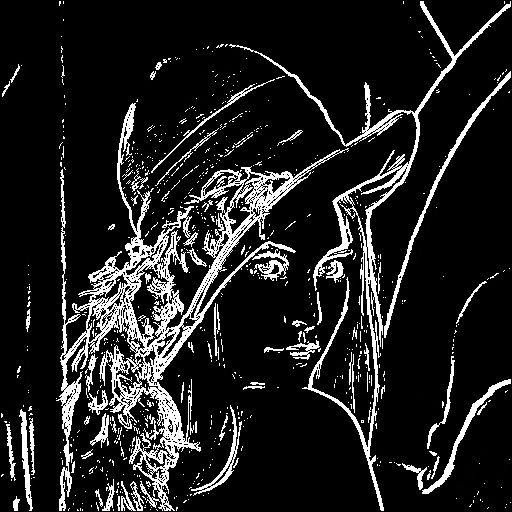
\includegraphics[scale=0.25]{Image/seuilHysteresis.png}
		\caption{Seuillage Hysteresis de Prewitt multidirectionnel	(\textit{Sb} = 44, \textit{Sh} = 60)}
		\label{fig:seuilHysteresis}
	\end{figure} 

	Cet algorithme permet de réduire le bruit et les trous dans les contours et donne d'excellents résultats.

	La difficulté de cette méthode est dans le choix des valeurs de \textit{Sb} et \textit{Sh}.
	Les mêmes problèmes que le seuillage fixe peuvent se produire. (voir \ref{fixe}).

	La complexité de cette algorithme est de \[n \times w \times h\]
	avec \textit{n} le nombre de passage sur l'image pour controler les pixel entre deux valeurs.

	Une fois, les contours bien définis par le seuillage, il reste encore une étape : l'affinage.


\section{Affinage}

\section{Conclusion}


\end{document}

%\begin{figure}[H]
%      \centering
 %     \includegraphics[scale=0.7]{Image/grandTableau.png} 
 %     \caption{Position de départ}
%      \label{fig:grandTableau}
%  \end{figure}

%	\[
%	\begin{pmatrix}
%	1 & 2 & 3 \\
%	4 & 5 & 6 \\
%	7 & 8 & 9
%	\end{pmatrix}
%	\]
